% Standalone source of the bubble time kernel of the second application example
% (Sec. 5), redrawn faithfully from the original bubble1 figure: a circular loop
% whose two propagators are distinguished by colour (teal upper, purple lower),
% single external legs running up and outward to P_1,P_2, vertex times beside the
% vertices, and parenthesised (momentum, mass) labels on each arc.
% Compile: pdflatex fig_bubble_diagram.tex   (included by paper.tex)
\documentclass[tikz,border=6pt]{standalone}
\usetikzlibrary{calc}
\definecolor{propgreen}{RGB}{0,161,150}
\definecolor{proppurple}{RGB}{121,90,188}
\begin{document}
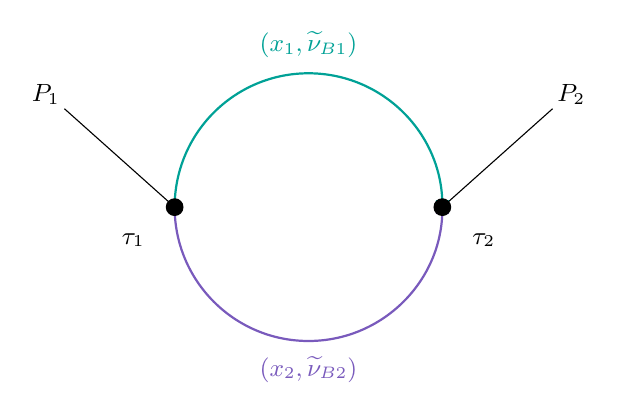
\begin{tikzpicture}[every node/.style={inner sep=1.5pt}]
  \coordinate (v1) at (-1.7,0);
  \coordinate (v2) at (1.7,0);
  % External legs running up and outward, with the energy sums at the tips.
  \draw (v1) -- (-3.1,1.25);
  \draw (v2) -- (3.1,1.25);
  \node[anchor=south east] at (-3.1,1.25) {\small $P_1$};
  \node[anchor=south west] at (3.1,1.25)  {\small $P_2$};
  % The two internal propagators: upper and lower halves of one circle, arrows
  % marking the momentum flow, coloured (momentum, mass) labels outside.
  \draw[->,thick,propgreen] (v1) arc[start angle=180,end angle=0,radius=1.7];
  \draw[->,thick,proppurple] (v1) arc[start angle=180,end angle=360,radius=1.7];
  \node[propgreen]  at (0,2.06) {\small $(x_1,\widetilde\nu_{B1})$};
  \node[proppurple] at (0,-2.06) {\small $(x_2,\widetilde\nu_{B2})$};
  % Vertex times beside the vertices, outside the loop.
  \node[anchor=east] at (-2.02,-0.42) {\small $\tau_1$};
  \node[anchor=west] at (2.02,-0.42)  {\small $\tau_2$};
  % Vertices last.
  \filldraw[fill=black,draw=black] (v1) circle (3pt);
  \filldraw[fill=black,draw=black] (v2) circle (3pt);
\end{tikzpicture}
\end{document}
